\documentclass{article}
\usepackage{graphicx}
\usepackage{pdfpages}

\begin{document}

\title{Extensions of L1 Trend Filtering: Seasonality, Outlier Modeling
and Other Effects with $l_1$ and $l_2$ Regularization}
\author{David Johnston}

\maketitle

\begin{abstract}
This paper extends and further elucidates ideas from Kim, Koh \& Boyd for L1 regularized
trend filtering and gives explicit formulas for reducing these problems down to
quadratic and linear programming problems that can be solved with various widely available
convex optimization libraries. We include seasonality effects with both
$l_1$ and $l_2$ regularization, outlier modeling, sparse level changes and
unequally spaced points. This paper also acts a documentation for the formulas used
in our open source python library \emph{myl1tf}
\footnote{https://github.com/dave31415/myl1tf}.
\end{abstract}

\section{The primary and dual quadratic programming problems}

We will start off at Section 5.2 of KKB where they state the quadratic programming problem for L1TF
and also state the dual problem.

\begin{eqnarray}
\mbox{minimize} & \frac{1}{2} ~ || y - x ||_2^2  + \lambda ||z||_1 \\
\mbox{subject to} & z = D x
\end{eqnarray}
The first is an $l_2$ norm and the second an $l_1$ norm. The Lagrangian, with a dual variable $\nu \in \mathbf{R}^{n-2}$, is
\[
L(x,z,\nu) =  || y - x ||_2^2  + \lambda ||z||_1 + \nu^T (D x -z)
\]


The dual function is
\[
\mbox{inf}_{x,z} ~ L(x,z,\nu) =
    \left\{
    \begin{array}{ll}
    - \frac{1}{2} ~ \nu^T D D^T \nu + y^T D^T \nu &  - \lambda \mathbf{1} < \nu < \lambda \mathbf{1} \\
  -\infty  & \mbox{otherwise.} \\
  \end{array}
  \right.
\]

since

\begin{equation}
\sup_\nu \inf_z \left(-\nu^T z + \lambda ||z||_1 \right) =
\left\{
    \begin{array}{ll}
   0 ~\mbox{if}~ |\nu| < \lambda \\
  -\infty  & \mbox{otherwise.} \\
  \end{array}
  \right. \label{eq:supinf}
\end{equation}
(see appendix for proof) and so the dual problem is

\begin{eqnarray}
\mbox{maximize} & -\frac{1}{2} ~ \nu^T D D^T \nu + y^T D^T \nu \\
\mbox{subject to} & - \lambda \mathbf{1} < \nu < \lambda \mathbf{1}
\end{eqnarray}

From the solution $\nu^*$ of the dual problem, we can compute the L1TF solution,
\[
x^* = y - D \nu^*
\]

\section{Seasonality}

As suggested by KKB we can adapt this to add a seasonal component.
\begin{eqnarray}
\mbox{minimize} & \frac{1}{2} ~ || y - x -s||_2^2  + \lambda ||z||_1 \\
\mbox{subject to} & z = D x \\
and & \sum_i^P s_i = 0\\
and & s_{i+P} = s_i
\end{eqnarray}

KKB does not go into detail on how to proceed with this and so we will begin here by deriving
the dual problem. We will do this by putting the constraints on $s$ directly into the
equation to be minimized.

To do this, we define $p$ to be the vector of independent variables defining the periodic components.
This vector has dimension $(P-1)$ as the $P$-th, dependent value is $-\sum_{i=1}^{P-1} p_i$ which enforces the constraint that
they sum to zero. This constraint is required if there is to exists a unique solution as otherwise one could add
any constant to $x$ and subtract it from $s$ without changing the model.

We can define $\tilde{p} \in \mathbf{R}^{P}$ as $\tilde{p} = \left( p,-\sum_{i=1}^{P-1} p_i \right) = T p$.
$T$ will be a $P \times (P-1)$ matrix with a $(P-1)$ identity matrix at the top and an extra row consisting of all -1.
The vector $s$ is now just a periodic re-cycling of $\tilde{p}$ which we can represent as s matrix $B$ which is formed by
row-wise stacking some number (ceil(N/P)) of $P \times P$ identity matrices and truncating rows to dimension $N$. So finally
we can write $s = B T p \equiv Q p$. By doing this we can rewrite the optimization problem as

\begin{eqnarray}
\mbox{minimize} & \frac{1}{2} ~ || y - x - Q p||_2^2  + \lambda ||z||_1 \\
\mbox{subject to} & z = D x
\end{eqnarray}
with the $p \in \mathbf{R}^{(P-1)}$ now unconstrained.

\subsection{Seasonality with $l_2$ regularization}

To improve stabilization and allow more control over $p$, we will add
a $l_2$ regularization constraint and write our problem.
\begin{eqnarray}
\mbox{minimize} & \frac{1}{2} ~ || y - x - Q p||_2^2  + \lambda ||z||_1 + \eta ~ \frac{1}{2} \tilde{p}^T \tilde{p}\\
\mbox{subject to} & z = D x
\end{eqnarray}

We will now proceed as before and derive the dual problem. To do this we first
write down the Lagrangian
\[
L(x,z,p,\nu,\eta,\lambda) =  R  + \lambda ||z||_1 + \nu^T (D x -z) + \eta ~ \frac{1}{2} p^T H ~p
\]
with  $H = T^T T$ and
\begin{eqnarray}
R & \equiv & || y - x - Q p||_2^2 \\
& = & \frac{1}{2} y^T y + \frac{1}{2} x^T x + \frac{1}{2} p^T Q^T Q p \\
&  & - y^T x - y^T Q p + x^T Q p
\end{eqnarray}

We can calculate $\mbox{inf}_{x,z,p} L(x,z,p,\nu,\eta,\lambda)$ by setting gradients w.r.t. $x$ and $p$ to zero. The
gradients of $R$ are

\begin{eqnarray}
\nabla_x R &  =  &  x^T - y^T - p^T Q^T\\
\nabla_p R &  =  &  \left( x^T - y^T - p^T Q^T \right) Q \\
& = & \left(\nabla_x R \right) Q \\
\end{eqnarray}
and the gradients of $L$ are
\begin{eqnarray}
\nabla_x L &  =  &  x^T - y^T - p^T Q^T + \nu^T D\\
\nabla_p L &  =  &  \left( x^T - y^T - p^T Q^T \right) Q + \nu p^T H \\
\end{eqnarray}


Setting $\nabla_x L$ =0 yields the equation.
\begin{equation}
y - x - Qp = D^T \nu \label{eq:residual}
\end{equation}
or
\[
x = y - Qp - D^T \nu
\]
Equation \ref{eq:residual} shows that $D^T \nu$ is the residual.
Setting $\nabla_p L$ =0 yields
\[
p = \eta^{-1} H^{-1} Q^T D^T \nu
\]
and we can use this last equation for $p$ to solve for $x$ and we can write these solutions as
\begin{eqnarray}
p^* & = &  \eta^{-1} H^{-1} Q^T D^T \nu \\
& and & \nonumber \\
x^* & = & y - D^T \nu - \eta^{-1} Q H^{-1} Q^T D^T \nu
\end{eqnarray}
and so once we have a solution for $\nu$ we can use these to obtain separate
solutions for $x$ and $p$.

The more subtle minimization w.r.t. $z$ will result in the same constraint in the dual problem as before. The reader
should ensure that they understand how the terms $\lambda ||z||_1 - \nu^T z$ result in the constraint
$- \lambda \mathbf{1} < \nu < \lambda \mathbf{1}$. One can show that outside of this range, the $inf_z$ of this term
is $-\infty$ (at either $z = \pm \infty$) and within is 0 (at $z=0$) (see appendix) and so any supremum for $\nu$
must lie within $|\nu| < \lambda$.

We then construct the dual problem by plugging these solutions into the Lagrangian and we arrive at
\begin{eqnarray}
\mbox{maximize} & -\frac{1}{2} ~ \nu^T A \nu + y^T D^T \nu \\
\mbox{subject to} & - \lambda \mathbf{1} < \nu < \lambda \mathbf{1}
\end{eqnarray}
with
\[
A = D D^T + \eta^{-1} D Q H^{-1} Q^T D^T
\]
We solve this quadratic programming problem as before for $\nu$ and then use the equations above
to calculate $x$ and $p$ from $\nu$. It is apparent that as $\eta \rightarrow \infty$ (seasonality is suppressed),
$p \rightarrow 0$ and we recover the same solution as before for $x$. We cannot use these equations directly with
the other limit $\eta = 0$, though we will address that in a later section. However there is no problem setting
$\eta$ to a neglibly small number and applying these formula.

\subsection{Seasonality using $l_1$ regularization}
We can also use an $l_1$ regularization term on the seasonality terms $p$ which will result in
sparse solutions for $p$. That is, with a well chosen regularization parameter,
no seasonality will be used when it isn't really required. This might be more useful than the $l_2$
regularization described above though the solution is a little more complicated.

The situation for $l_1$ regularization is similar to the above for the $x$ coordinate and leads to the
same Equation \ref{eq:residual} for the residual. Submitting this solution for $x$ in terms of $\nu$ and $p$
leads to an optimization problem for $\nu$ and $p$ as follows

\begin{eqnarray}
sup_{\nu} ~ inf_p & -\frac{1}{2} ~ \nu^T D D^T \nu + y^T D^T \nu -\nu^T D Q p + \eta ||T p||_1 \\
\mbox{subject to} & - \lambda \mathbf{1} < \nu < \lambda \mathbf{1}
\end{eqnarray}

We can write $||T p||_1 = ||p||_1 + |u^T p| $ where $u$ is the unity vector $u_i=1$. There are no constraints on
$p$ so this term $|u^T p|$ can be any non-negative number for some choice of $p$ and so
$inf_{p} ~  -\nu^T D Q p + \eta ||T p||_1 = inf_{p} ~  -\nu^T D Q p + \eta ||p||_1 $ and
\[
inf_{p} ~  -\nu^T D Q p + \eta ||p||_1 =
    \left\{
    \begin{array}{ll}
    0 &  - \eta \mathbf{1} <  Q^T D^T \nu < \eta \mathbf{1} \\
  -\infty  & \mbox{otherwise.} \\
  \end{array}
  \right.
\]

This implies that the Lagrangian for $\nu$ to be optimized is the same as the non-seasonal
version but with an additional constraint.

\begin{eqnarray}
\mbox{maximize} & - \frac{1}{2} ~ \nu^T D D^T \nu + y^T D^T \nu \\
\mbox{subject to} & - \lambda \mathbf{1} < \nu < \lambda \mathbf{1} \\
& - \eta \mathbf{1} < Q^T D^T \nu < \eta \mathbf{1} \\
\end{eqnarray}

Notice that the $l_2$ solution leads to a modification of the quadratic form whereas the
$l_1$ problem instead leads to an additional constraint. Both of these are standard quadratic
programming problems that can be solved with any convex optimization library (such as cvxopt for python).
A difference however is that the $l_2$ solution included a simple way of calculating $x$ and $p$ once
$\nu$ has been solved.

With the $l_1$ solution here, we have to solve a second optimization problem
in order to separate out the separate components. To do this, note that after $\nu$ has been solved for,
the first $\chi^2$ term is now constant
and so we need to optimize the sum of regularization terms by themselves

\begin{eqnarray}
\mbox{minimize} & ||D x||_1 + (\eta / \lambda) ||T p||_1 \\
\mbox{subject to} & y - x - Qp = D^T \nu \\
\end{eqnarray}

which we can write solely in terms of $p$ as

\begin{eqnarray}
\mbox{minimize over} ~p : & ||D (y - D^T \nu - Q p)||_1 + (\eta/\lambda) ||T p||_1 \\
\end{eqnarray}

The trick to solving this is to combine these into a larger vector space
\[
w = [D (y - D^T \nu), 0]^T
\]
and the $F$ matrix defined by two matrix blocks
\begin{equation}
F=\left[
\begin{array}{c}
D Q  \\
\hline
(\eta/\lambda) T \\
\end{array}\right]
\end{equation}

and write this as
\begin{eqnarray}
\mbox{minimize over}~ p : & ||w-F p||_1 \\
\end{eqnarray}

This is now in the form of a well known problem, the Least Absolute Deviation (LAD) problem and can be written as a
a linear program. The cvxopt library contains a program for solving this problem. Thus,
we can solve for $\nu$ by solving the quadratic programming problem and then solve this equation for $p$ and then
use Equation \ref{eq:residual} to solve for $x$.

\section{Modeling outliers and step functions for more robust fits}
KKB also suggest including outliers by adding terms $u$ to the model with a strong $l_1$ regularization. This will
result in a sparse solution for the $u$ values which can model things like spikes without throwing off the other terms.
These can be treated just like the $l_1$ regularized seasonality and will result in the same quadratic programming
problem as before with an additional constraint $-\delta < D^T \nu < \delta$ where delta is the $l_1$
regularization parameter for the $u$ vector.

As before, we end up with a solution for $\nu$ and must still solve the LAD problem to get separate solutions for
$x, p$ and $u$.
\begin{eqnarray}
\mbox{minimize over} ~p,u : & ||D (y - D^T \nu - Q p - u)||_1 + (\lambda / \eta) ||T p||_1 + \delta/\lambda ||u||_1 \\
\end{eqnarray}

We can employ the same trick as before and write this as a single LAD problem on a larger vector space.
\begin{eqnarray}
\mbox{minimize over}~ p,u : & ||w-F z||_1 \\
\end{eqnarray}
with
\begin{eqnarray}
z & = & [p , u]^T\\
w & = & [D (y - D^T \nu), 0, 0]^T \\
\end{eqnarray}
and $F$ specified by matrix blocks
\begin{equation}
F=\left[
\begin{array}{c|c}
D Q  & D   \\
\\
\hline
& \\
(\eta/\lambda) T & 0_{P \times n} \\
\\
\hline
& \\
0_{n \times P-1}, & (\delta/\lambda) I_n \\
\end{array}\right]
\end{equation}

\subsection{Step functions}

Rather than spikes ($\delta$-functions) we can also consider step functions (or Heaviside functions).
The solution is nearly identical to the above except that we replace matrix $D$ in the upper right
hand corner with $D H$ where $H$ is the matrix with 1 in it's upper triangle and diagonal and zero
in it's lower triangle. This is because step functions are simply cumulative sums of delta functions.

With both spikes $u$ and step function transitions $h$ (regularized by $\gamma$), we can write the
equations

\begin{eqnarray}
z & = & [p , u, h]^T\\
w & = & [D (y - D^T \nu), 0, 0, 0]^T \\
\end{eqnarray}
and $F$ specified by matrix blocks
\begin{equation}
F=\left[
\begin{array}{c|c|c}
D Q  & D  & D H \\
&\\
\hline
&\\
(\eta/\lambda) T & 0_{P \times n} & 0_{P \times n}\\
&\\
\hline
&\\
0_{n \times P-1} & (\delta/\lambda) I_n & 0_{n}\\
&\\
\hline
&\\
0_{n \times P-1} & 0_n & (\gamma/\lambda) I_n \\
\end{array}\right]
\end{equation}

By now, one should notice the pattern that adding any new $l_1$ regularization
terms simply requires a modification of the above equations which just requires
that one express the intentions in matrix form.

\section{L1 norms for everything}

Rather than using an $l_2$ on the residual we can use an $l_1$ term for this and so use
$l_1$ norms for everything. An $l_1$ norm on the residual is another way of giving less
weight to outliers. It also simplified the solution as there is no quadratic programming
problems to solve. We can use the same trick of writng the whole optimization as a single
LAD problem in a higher dimensional space.

Minimize the following for $x$, $p$ and $h$:
\begin{equation}
||y - x - Q p -H h||_1 + \lambda_2 ||D_2 x|| + \lambda_1 ||D_1 x - g||
+ \eta ||T p||_1 + \delta ||h||_1
\end{equation}

Here we are considering first and second derivatives: matrices $D_1$ and $D_2$ plus the seaosnality
term and level changes. In addition we allow for $g$ a non-zero preferred first derivative. As before
we can write this as a single LAD problem:
\[
\mbox{minimize over}~ z :  ||w-F z||_1 \\
\]
where

\begin{eqnarray}
z & = & [x, p , h]^T\\
w & = & [y, g, 0, 0, 0]^T \\
\end{eqnarray}
and $F$ specified by matrix blocks
\begin{equation}
F=\left[
\begin{array}{c|c|c}
I_n  & Q  & H \\
&\\
\hline
&\\
-\lambda_1 D_1 & 0_{m \times (P-1)} & 0_{m \times n}\\
&\\
\hline
&\\
-\lambda_2 D_2 & 0_{m \times (P-1)} & 0_{m \times n}\\
&\\
\hline
&\\
0_{P \times n} & -\eta T & 0_{P \times n} \\
&\\
\hline
&\\
0_{n} & 0_{n \times (P-1)} & -\delta I_n
\end{array}\right]
\end{equation}


\section{Implementation}
The Githib repository https://github.com/dave31415/myl1tf contains an implementation for this
L1TF modeling with seasonality. This was a fork of the repository
https://github.com/elsonidoq/py-l1tf by Pablo Zivic which implements the
simpler version without seasonality and other effects. Both versions are in python and
use the python cvxopt library to solve the convex optimization problems. Our
version contains some test programs as well. For example, the following command,
\begin{verbatim}
test_myl1tf.test_l1tf_on_mock_with_period(period=6, eta=1.0,alpha=0.5)
\end{verbatim}
creates a mock data-set, fits the model and displays the following plot.
\begin{figure}
\centering
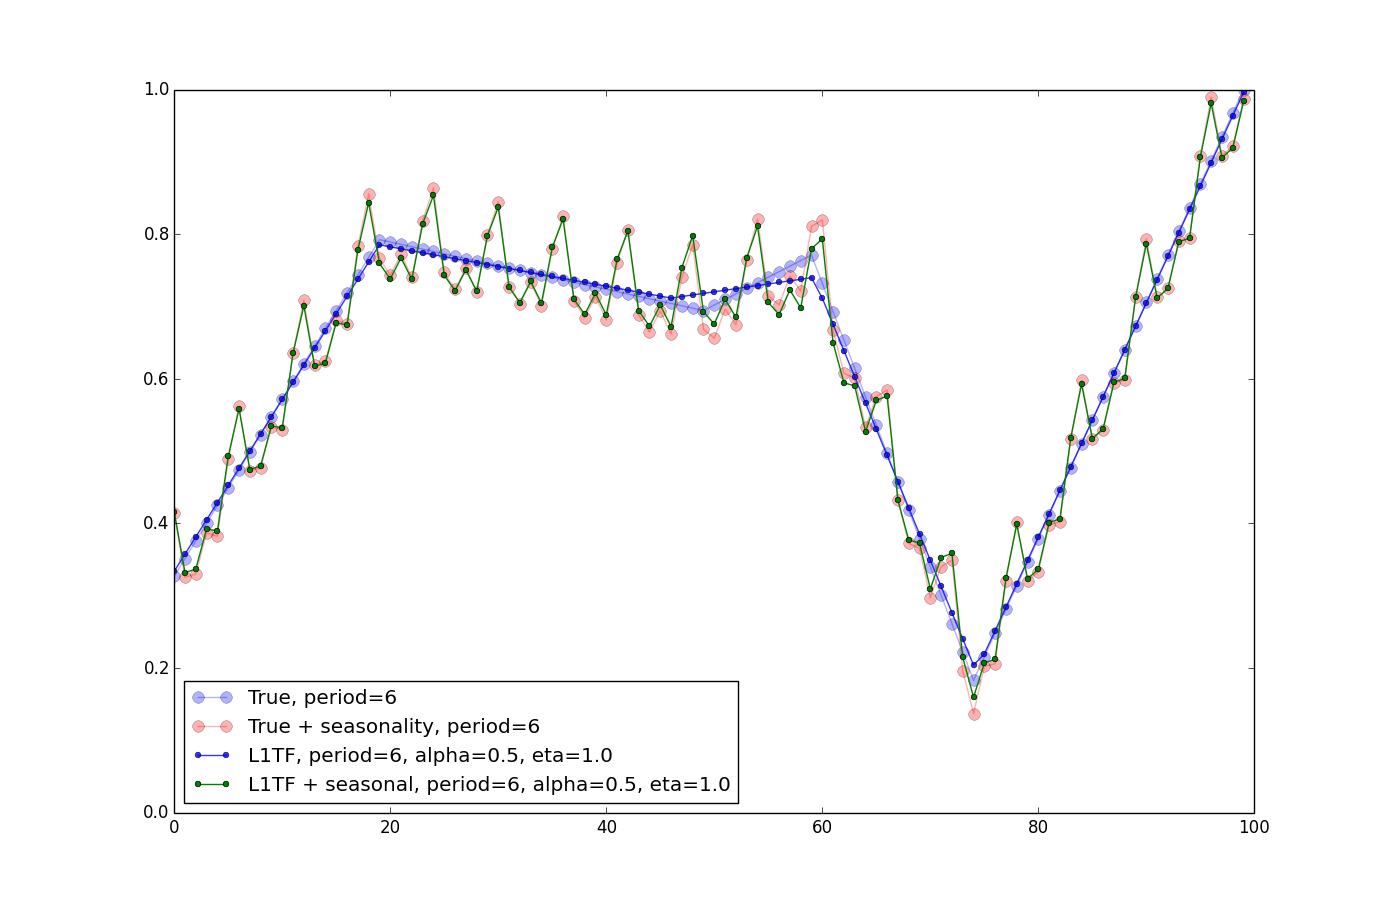
\includegraphics[width=500pt]{example.png}
\end{figure}
(Note \emph{eta} = $\eta$ and \emph{alpha} = $\lambda$ as \emph{lambda} is a reserved word in python).

\section{Appendix}
\subsection{Calculating the derivative matrices for unequally spaced points}

The first and second derivatives of unequally spaced data points can be calculated, at those data points,
as follows. We can use Lagrange's interpolation formula to fit the unique quadratic function through any
three points $(x_1,y_1), (x_2,y_2), (x_3, y_3)$.

\begin{eqnarray}
P(x) & = & \sum_{i=1}^{3} y_i P_i(x) \\
P_i(x) & = & \prod_{j=1, j \ne i}^{3} \frac{\left( x-x_j \right)}{ \left( x_i - x_j \right)}
\end{eqnarray}

Written out in full this is
\begin{eqnarray}
P(x) & = & y_1 \left(\frac{x-x_2}{x_1-x_2}\right) \left( \frac{x-x_3}{x_1-x_3}\right) \nonumber \\
     & + & y_2 \left(\frac{x-x_1}{x_2-x_1}\right) \left( \frac{x-x_3}{x_2-x_3}\right) \nonumber \\
     & + & y_3 \left(\frac{x-x_1}{x_3-x_1}\right) \left( \frac{x-x_2}{x_3-x_2}\right) \nonumber
\end{eqnarray}
The first derivative is
\begin{eqnarray}
\frac{dP}{dx} & = & y_1 \frac{\left(2x-x_2-x_3 \right)}{\left(x_1-x_2\right)\left(x_1-x_3\right)} \nonumber \\
     & + & y_2 \frac{\left(2x-x_1-x_3 \right)}{\left(x_2-x_1\right)\left(x_2-x_3\right)} \nonumber \\
     & + & y_3 \frac{\left(2x-x_1-x_2 \right)}{\left(x_3-x_1\right)\left(x_3-x_2\right)} \nonumber
\end{eqnarray}
and second derivative is

\begin{eqnarray}
\frac{d^2P}{dx^2} & = & y_1 \frac{2}{\left(x_1-x_2\right)\left(x_1-x_3\right)} \nonumber \\
     & + & y_2 \frac{2}{\left(x_2-x_1\right)\left(x_2-x_3\right)} \nonumber \\
     & + & y_3 \frac{2}{\left(x_3-x_1\right)\left(x_3-x_2\right)} \nonumber
\end{eqnarray}

We are only interested in evaluating these at the middle point $x=x_2$. The second derivative is
indpendent of $x$ anyway but the first derivative evalued at $x=x_2$ is

\begin{eqnarray}
\frac{dP}{dx}(x=x_2) & = & y_1 \frac{\left(x_2-x_3 \right)}{\left(x_1-x_2\right)\left(x_1-x_3\right)} \nonumber \\
     & + & y_2 \frac{\left(2x_2-x_1-x_3 \right)}{\left(x_2-x_1\right)\left(x_2-x_3\right)} \nonumber \\
     & + & y_3 \frac{\left(x_2-x_1 \right)}{\left(x_3-x_1\right)\left(x_3-x_2\right)} \nonumber
\end{eqnarray}

If we assume that the $x_i$ are sorted to be increasing and there are no duplicates, this can be
written in matrix form, with first and second derivative matrices $F$ and $D$ being
block diagonal with block length 3 and specified by the last two equations.

For equally spaced points of unit separation, i.e. $x_2 = x_1 +1$ and $x_3 = x_1 + 2$ they reduced to the
usual formulas for finite difference derivatives,
$F = BlockDiag((-0.5,0,0.5))$ and $D = BlockDiag((1,-2,1))$. These results for unequally spaced
points should give results exactly equal to analytical calculations when evaluated on quadratic, linear
or constant functions. These two facts provides a useful test for any implementation.

\subsection{Proof of Equation \ref{eq:supinf}}

We wish to prove that
\begin{equation}
\sup_\nu \inf_z \left(-\nu^T z + \lambda ||z||_1 \right) =
\left\{
    \begin{array}{ll}
   0 ~\mbox{if}~ |\nu| < \lambda \\
  -\infty  & \mbox{otherwise.} \\
  \end{array}
  \right.
\end{equation}

Note that this equation is proven if we prove it for each component that is summed so
we can drop vector notation and treat them as scalars.

First define $f(\nu) = \inf_z \left(-\nu z + \lambda |z| \right)$. Notice the important fact
that $f(\nu) = f(-\nu)$ because if the $\inf$ is achieved at $z$ for some $\nu$ then the same
$\inf$ can be achieved at $-z$ for $-\nu$. Thus it is symmetric in $\nu$, $f(\nu) = f(|\nu|)$.
Note also that $f(0) = 0.$

Now let's consider the case $|\nu| \le \lambda$. Clearly $\nu z \le |\nu z|$ so
$f(\nu) = \inf_z \left(-\nu z + \lambda |z| \right) \ge  \inf_z \left(|z| (-|\nu| + \lambda) \right)
\ge 0$. So $f(\nu) = 0$.

Now consider the other case $|\nu| > \lambda$. Now for any positive $z$,
$f(\nu) < \left((-\nu + \lambda) |z| \right)$ which has $inf_z = -\infty$.


\section{References}
S.-J. Kim, K. Koh, S. Boyd, and D. Gorinevsky
SIAM Review, problems and techniques section, 51(2):339–360, May 2009.\\
http://stanford.edu/\~boyd/papers/pdf/l1\_trend\_filter.pdf


\end{document}

